\section{Investigation of the Current System}
This section details the in-depth investigation that was performed on the current quiz system used by the school. Initial contact with the school was made via an email to one Mr Nick Bucknall, currently head of Year 8, on the 30th June 2015. Following a brief email exchange, the details of which can be found below, Below can be found the different aspects that were investigated.

% \subsection{Overview of System}
% Currently, the school does not have a formal, standardised system in place. A somewhat ad-hoc approach is currently used, using a combination of emails, documents scattered across the network, and verbal communication. Obviously, this approach has a number of issues, the details of which can be found below in the observations performed, as well as the analysis of the current system's limitations.

% Import interviews
\input{./tex/analysis/current_system/intervews.tex}

% Import questionnaires
\subsection{Questionnaires}

An online questionnaire was created for students of the school to fill in, detailing their opinion on form times, how it could be improved through the use of quizzes.

\subsubsection{Questions}
The following questions were included	 on the questionnaire, distributed to students at the school:

\noindent\fbox{%
    \parbox{\textwidth}{%
        \begin{enumerate}[leftmargin=0cm,itemindent=.5cm,labelwidth=\itemindent,labelsep=0cm,align=left]
					\item How satisfied are you with your current form time experience? 1 2 3 4\\
					\item ``My form times are always well structured.'' How far do you agree or disagree with this statement? 1 2 3 4 5\\
					\item Out of the following activities you selected, which do you enjoy the most?
								\begin{itemize}
									\item Silent reading
									\item Knowledge quiz
									\item Group discussion
									\item Board games
									\item Physical activities
									\item Other\\
								\end{itemize}
					\item Approximately how often do quizzes feature in your form times? 1 2 3 4\\
					\item ``My form times would be improved if we did quizzes more often.'' How far do you agree or disagree with this statement? 1 2 3 4\\
					\item ``I find that quizzes improve the relationship between me and the rest of my form'' How far do you agree or disagree with this statement? 1 2 3 4\\
					\item Which topics have you been given quizzes on? Select all that apply.
								\begin{itemize}
									\item General knowledge
									\item Media
									\item Sports
									\item History
									\item Literature
									\item Relationships
									\item Brainteasers
									\item Other\\
								\end{itemize}
					\item To what extent do you interact with other forms in your year during form time? 1 2 3 4\\
					\item Do you believe form times would be improved by interaction with other forms? Yes No\\
					\item If you wish, please expand on your answer to the previous question.
				\end{enumerate}
    }%
}

\subsubsection{Results}
The following results were collected after the quiz had been live for 10 days. They were automatically generated using the 

% Import observations
\subsection{Observations}

Having been a member of the school community for over five years, I am well placed to provide an observation on how the school currently goes about creating, setting and analysing quizzes used in form times. Currently, no formal system is in place; an ad-hoc system is used, following this general pattern:

\begin{enumerate}
	\item The head of year creating the quiz thinks of a set of questions and possible answers, usually following a theme, and then writes them down on a Microsoft Word document. The correct answer is marked out, to aid the form tutor in marking the quiz. This document is then saved to a drive on the school's LAN.

	\item The head of year then notifies the individual form tutors of the quiz, usually at one of their weekly meetings, and tells them to conduct the quiz with their form group on a certain date.

	\item When the date is reached, the form tutor opens the document from the network, ensuring that the document is kept hidden to avoid members of the form viewing the correct answers.

	\item The form tutor reads each question out in turn, and the members of the form work together to attempt to work out the answer. They either come up with their own answer or choose from a list of options, depending on whether or not the question is multiple choice. The form tutor marks down the answer they chose, and this process repeats until the quiz is completed.

	\item Once all the questions have been answered, the form tutor adds up the total number of marks achieved by the form.

	\item The form tutor then passes the mark onto the head of year, either by email or when passing them in the corridor or the staffroom. This task is sometimes performed by a member of the form themselves, occasionally with the expectation that the mark achieved will be exaggerated somewhat.

	\item After receiving all the results, the head of year works out which form achieved the highest result, and which the lowest. This result is reported back to the year in the weekly assembly, often with a small reward for the highest achieving form.
\end{enumerate}

% Import document inspections
\subsection{Document Inspections}

A number of documents were collected from the school, relating to both how the quizzes are currently set, and the management structure of the school; these will aid in creating the best possible solution that fits the needs of the school.

\subsubsection{Weekly Email} % (fold)
\label{ssub:weekly_email}
\begin{figure}[h!]
  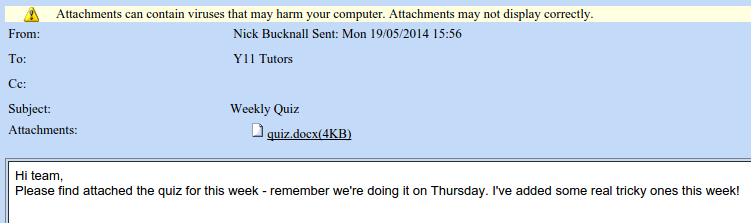
\includegraphics[scale=0.46]{analysis/current_solution/document_inspections/email}
  \caption{Email sent by Nick Bucknall on the 19th May 2014}
\end{figure}

This capture of an email sent by Nick Bucknall (a head of year, soon to be head of house) to his tutor team demonstrates the inefficiency with which the quiz system is currently handled. Sending an email with an attachment once a week is an approach fraught with issues, the most glaring of which is the shocking lack of organisation. As can be gleaned from the shot, the school's email system is not the most modern, and this can make it difficult to find particular emails - such as the weekly quiz. A far better solution would be to have the correct quiz appear automatically.
\clearpage
% subsubsection weekly_email (end)

\subsubsection{Weekly Quiz} % (fold)
\label{ssub:weekly_quiz}
\begin{figure}[h!]
  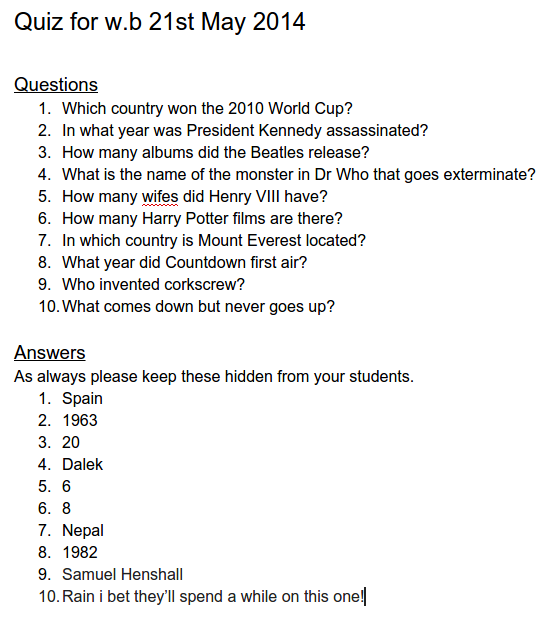
\includegraphics[scale=0.55]{analysis/current_solution/document_inspections/quiz_sample}
  \caption{Quiz created by Nick Bucknall on the 14th May 2014}
\end{figure}

The above capture of a quiz created by Nick Bucknall, and distributed to form tutors, demonstrates the form that that the quizzes currently take. As can be discerned, though the current method undoubtedly works, the existence of the answers so close to the questions causes a number of difficulties; most notably, it means that the questions must be read out by the form tutor, and the actual question sheet cannot be shown. Additionally, it no doubt takes time for Nick Bucknall to lay out the document in such a manner each week; a better solution would be if a standard template could be used (though not, it should be noted, in the form of another word processed document).
\clearpage
% subsubsection weekly_quiz (end)



% Import similar systems
\subsection{Similar Systems}
There are a number of systems available, both free and at a cost, that would allow the school to improve their current method of quiztribution (\textit{quiz distribution}). Several popular options are outlined below.

\subsubsection{Quiz Creation Websites}
A number of websites exist that allow users to design, play and share their own quizzes. These websites, including \textit{QuizWorks}, \textit{ExamTime} and \textit{QuizBean} generally follow the same pattern: the user creates an account, is directed to an interface wherein they can design a quiz, and is then given a link with which they can share the quiz with others. For basic quiz creation, these websites are free, though for more advanced usage (\textit{QuizWorks} defines an ``advanced'' quiz as one containing more than 15 questions), paid plans are available.

As these systems are websites, they can be accessed from practically any computer or mobile device, as long as there is an internet connection in range. This means that users can continue to work on their quizzes, whether designing or answering them, outside of their place of work.

Though these systems are undoubtedly useful, and could, with a few compromises, be easily integrated into the school's routines, they lack an awareness of the structure of a school. There is no concept of ``form groups'' or ``heads of year'', both are which are vital concepts if the system is to meet what the school desires. Additionally, they lack the ability to display a detailed analysis of the results (at least, not without paying a somewhat exorbitant fee - \pounds60 per month in the case of \textit{QuizWorks}), a side effect of their focus on individuals as opposed to groups.

\subsubsection{Quiz Creation Software Packages}
Similar to quiz creation websites, quiz creation software packages allow the user to design and play a quiz. However, these systems are desktop applications (the majority are designed for Microsoft Windows), and so can only be accessed from a single desktop or laptop system. Examples of these systems include \textit{Wondershare Quiz Creator}, \textit{Tanida QuizBuilder}, and \textit{Articulate Storyline 2}. Unlike the mostly free websites, these software packages are often very expensive: the three systems mentioned range in price from \$99 - \$1846 for a single license, with additional licenses costing even more.

To compensate for the high prices, these desktop applications contain a vast feature set. Quizzes of every imaginable type can be created, from drag-and-drop, multiple choice, word bank quizzes, and many more. Images can be included, points assigned, and complex animations can be set to make the quiz as visually appealing as possible. In addition, reports can be generated with tremendous amounts of data, showcasing practically every data point imaginable.

Useful though these features are, they are a touch overkill for what the school's purposes. The systems are not the easiest things to use in the world, something that, considering the teacher's relative lack of IT skills, is quite a drawback. Additionally, the high costs make the systems prohibitively expensive, considering the school's status as the worst funded school in the county.

\subsubsection{Quizdom}

% Import justification of methods
\subsection{Justification of Methods}

Methods will be justified soon.

% Import IPSO chart
\subsection{IPSO Chart}
This IPSO chart describes the inputs, outputs, storage locations and general processes that are associated with the system.

\begin{table}[h]
\centering
\begin{tabular}{|l|l|}
\hline
\multicolumn{1}{|c|}{{\bf Inputs}}                                                                                                                              & \multicolumn{1}{c|}{{\bf Processes}}                                                                                                                                                                                                                                                                         \\ \hline
\begin{tabular}[c]{@{}l@{}}Full name\\ Password\\ \\ Form name\\ \\ Quiz title\\ Quiz questions\\ Quiz answers\\ Forms the quiz should be sent to.\end{tabular} & \begin{tabular}[c]{@{}l@{}}Create HOY accounts from inputs\\ Create form group accounts\\ \\ Create and store quizzes\\ \\ Allow quizzes to be answered by\\ forms and store answers.\\ \\ Prevent quizzes from starting unless\\ all forms have joined.\\ \\ Mark quizzes and analyse results.\end{tabular} \\ \hline
\multicolumn{1}{|c|}{{\bf Storage}}                                                                                                                             & \multicolumn{1}{c|}{{\bf Outputs}}                                                                                                                                                                                                                                                                           \\ \hline
\begin{tabular}[c]{@{}l@{}}Store user accounts\\ Store individual quizzes with answers.\\ Store mark for quizzes.\\ Store analysis of results.\end{tabular}     & \begin{tabular}[c]{@{}l@{}}Quiz containing questions and answers.\\ Analysis of quiz results.\end{tabular}                                                                                                                                                                                                   \\ \hline
\end{tabular}
\caption{IPSO Chart}
\label{my-label}
\end{table}

% Import limitations of current system
\subsection{Limitations of Current System}
There are evidently a large number of issues with the above method. Firstly, distributing the quizzes via a word-processed document is not a particularly efficient method. It results in the network drive being cluttered with a variety of documents, perhaps with a non-existent naming scheme. This makes it harder for the form tutors to find the correct quiz for the week, slowing the whole process down. A more effective solution would be to have everything in it's own self contained system, with its own dedicated quiz screen, which points out the correct quiz to the tutors.

Additionally, having the questions and possible answers on the same document puts the integrity of the quiz at risk. Currently, form tutors get around this by hiding the document, but this can cause complications where students forget the possible answers, as well as other issues. It word be far more effective to always have the quiz displayed on screen on the interactive whiteboard, but the current system prohibits this.

Often, teachers forget about the quiz altogether, or believe it to be on a different date than when it is actually scheduled. This is a relatively common occurrence, and means that the quiz either has to be rescheduled (which those tutors who did remember find annoying), or that particular form has to miss out on the quiz that week; this can damage their overall reputation in the school community. A dedicated system could provide them a notification, perhaps via an email, that they should hold the quiz that afternoon. Additionally, the system could be set up in such a way that the quiz only begins once all the appropriate forms have connected.

Furthermore, the current system is not particularly fair. Students can spend as long as they wish on a single question, as long as the quiz is completed within the 25 minutes given to the form time. It would be fairer if the form was given a time limit of, say 60 seconds, after which the system automatically moves on to the next quiz.

The current system is also very isolated. Following the appointment of the new principal, the school has sought to implement the principle of ``togetherness'', whereby students work together more often. Though the current quiz system aligns itself with this philosophy to a degree (each form works together to come up with the answer), it could be improved by allowing a degree of interoperability between the forms. For example, if a quiz was being answered by all the forms in Year 8, one form could be given the opportunity to pose a question to the other forms, perhaps referencing one of the jokes sanctioned by the school.

By allowing the form tutors themselves to mark the quiz, their is a large risk of
inaccurate results being reported back, possibly altered in such a way that favours the form. Though this allows the head of year to display trust to his team of form tutors, there exists in the school a very competitive atmosphere, increasing the chance that such malpractice will occur. A safer approach would be to allow the system to mark the form's answers, and then report this directly to the head of year.

Though the heads of year throughout the school possess many fine and admirable qualities, it would be remiss to apply to them the label of ``mathematician''.  For simply calculating the best and worst performing forms for any given quiz, there are few issues with the current system (though it would be convenient if this was worked out automatically). It is when attempting to work out more complex results, such as the average score of a form over a period of several years, that the humble head of year falls short. A dedicated system would be able to perform a complicated analysis on the entire set of data it collects, allowing for a far more interesting report to be generated. This data could then be presented at an end of year, or even school, assembly, showcasing the best form in each category (or some other arbitrary statistic) throughout their entire school career.

Finally, the fact that the school is completely replacing the head of year system with new heads of house means that the entire approach
